% Não sei se fica esse título mesmo... +- 2 páginas
% Conteúdo
% - Estatísticas do time

% - Desempenho usando a técnica do Hulk e sem o Hulk - comparação entre nossos times e nosso time contra Python-DTU 
%Hulk: it is the agent responsible for buying;

% - Desempenho usando 1 morrinho ou 2 morrinhos: uso dessa técnica contra o time chinês



% Vantagens e desvantagens.

\section{Results}
%será que devia dizer porque perdemos?%. 
We have tried to develop a system as complete as possible and we created several strategies for each system feature, like exploring, exploiting, buying, repairing, and attacking. Hence we developed many versions of the system, we exhaustively tested each one against the others to select the more efficient. We also tested our system during the contest test phase against the teams provided by the contest organisation. This approach was our main advantage in the contest and one of the reasons we played eighteen matches against six different opponents and won seventeen. However our system has a worse performance when it confronts a passive system because it is not so offensive. If our agents are in a good map zone they do not bother about the opponent: they assume that the opponent is not in a good area. Also, our agents have no focus on defending a conquered zone and this explains the match we lost against Python-DTU during the contest.

Two main strategies were responsible for the good performance of our system: the buying and exploitation strategies. The buying strategy was decisive because it forced our opponents to reinforce their agents spending a lot of their money. In a match against Python-DTU during the tests phase, for example, we conquered a small area but we won because we had more money. Fig.~\ref{hulk1} shows the achievement points from this match. In the step 175 the Python-DTU (in blue) spent most of their money strengthening their agents and SMADAS (in green) spent only a part of its money. In the last 400 steps, from the step 350 to the 750, we had about 23 achievement points in each step, summing 9200 achievement points. In the end, this difference allowed us to win this match, as shown in Fig.~\ref{hulk2}.

%\begin{figure}
%\centering 
%	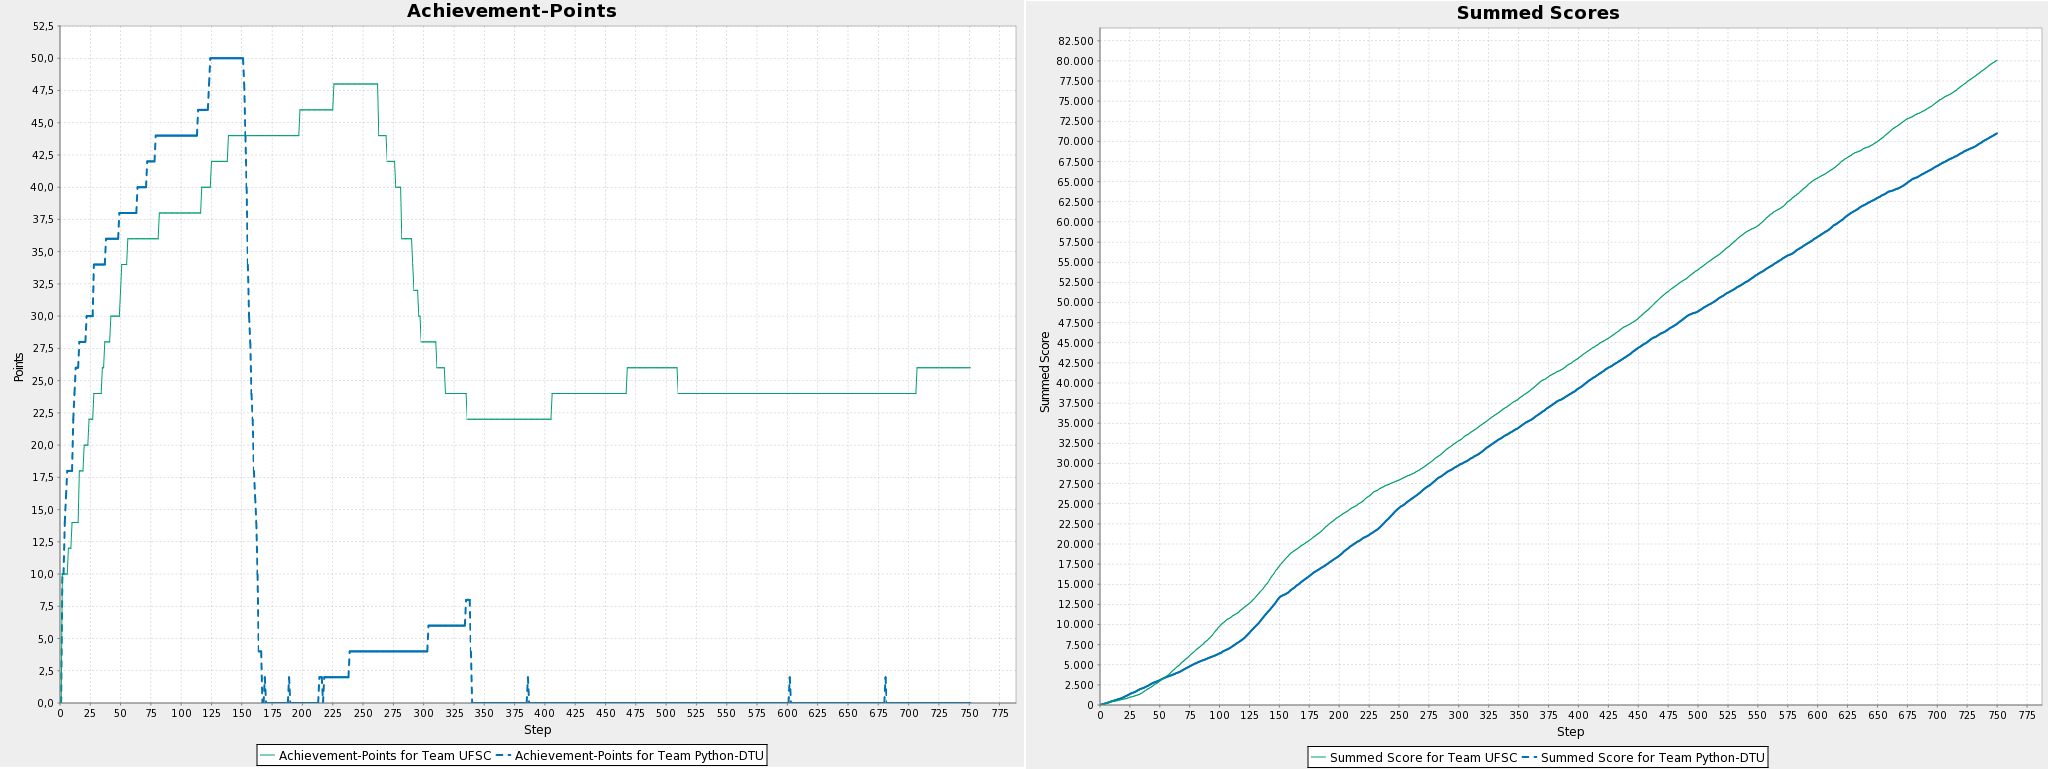
\includegraphics [width= 12cm] {./AchievementPoints.png}
%	\caption{From the step 350, SMADAS-UFSC (in green) has more achievement points than Python-DTU (in blue) (a). This difference has decided the match for SMADAS-UFSC system (b).}
%\label{fig:achievementpoints}	
%\end{figure}


\begin{figure}
	\centering
	\subfloat[]{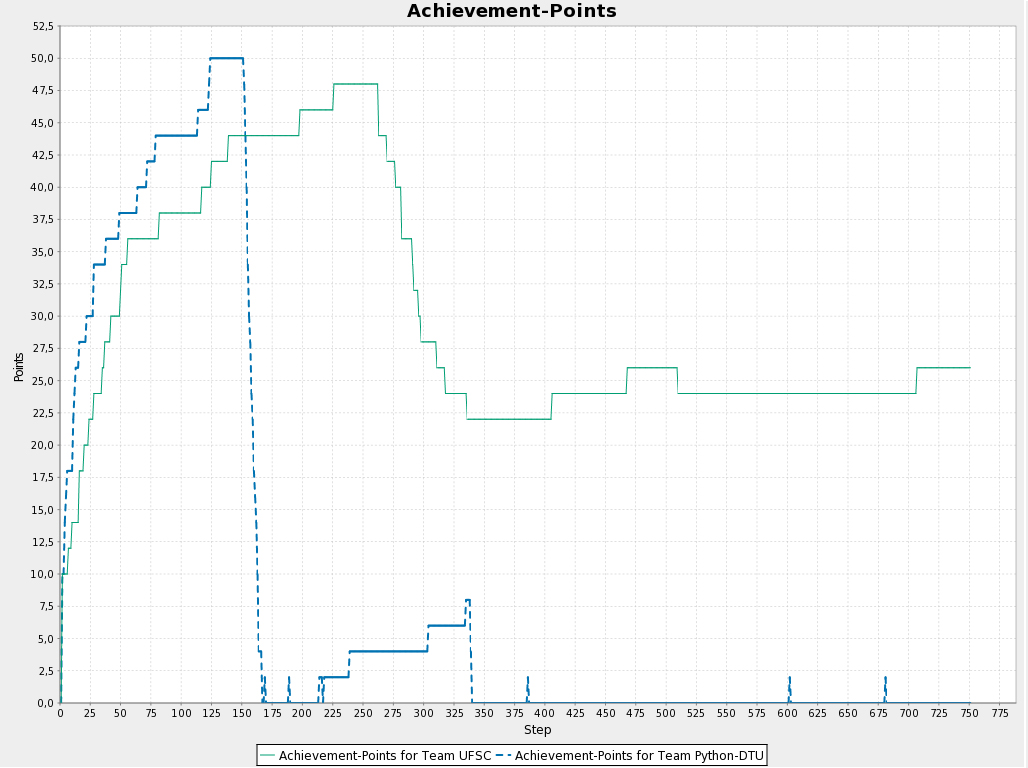
\includegraphics[width=0.48\linewidth]{./hulk1.jpg}\label{hulk1}}
	\hspace{0cm} % este comando é para deixar uma distância de 1 cm entre as figuras
	\subfloat[]{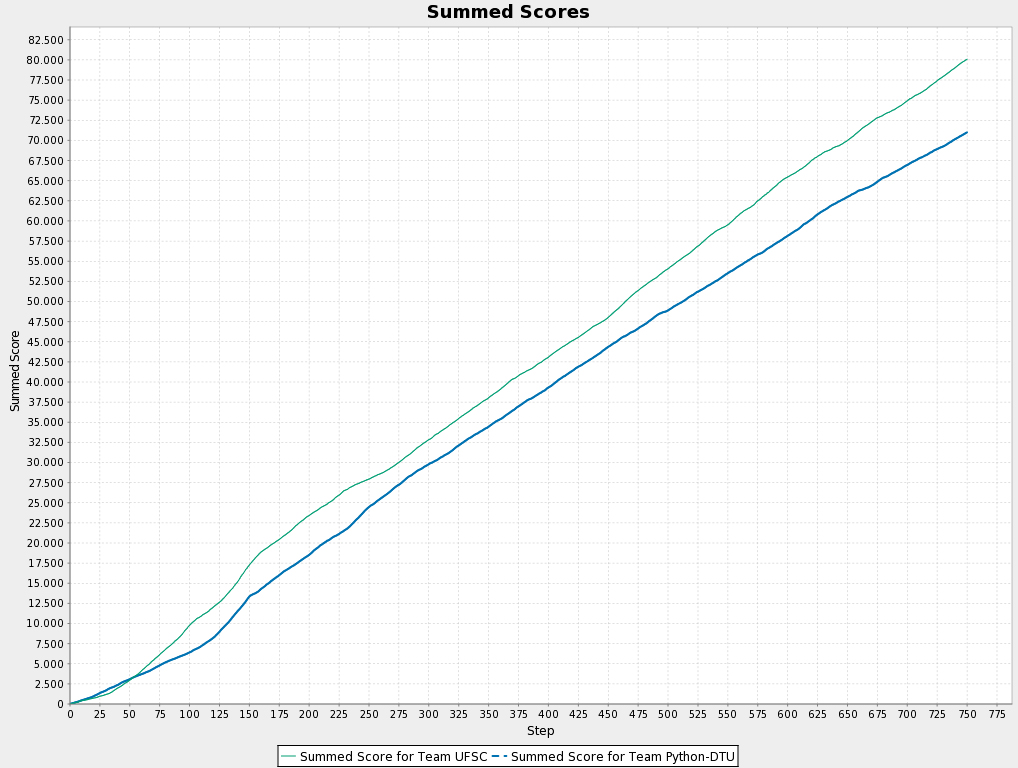
\includegraphics[width=0.48\linewidth ]{./hulk2.jpg}\label{hulk2}}
	\caption{From the step 350, SMADAS-UFSC (in green) has more achievement points than Python-DTU (in blue) (a). This difference has decided the match for SMADAS-UFSC system (b).}
	\label{fig:achievementpoints}
\end{figure} 

Our exploitation strategy chooses two good zones in the map. It was efficient because usually the opponents are concerned about finding and conquering just one good zone. Thus while part of our agents are under attack in one of these zones, the other part are scoring in another zone. This strategy earns less points in each step, because our agents are divided in two smaller zones, but it has better results against an offensive opponent.  Fig.~\ref{fig:1x2morrinho} shows a comparison from our system performance using these two exploiting strategies. The system in green tries to conquer one single zone and the blue system looks for two zones. The blue system has fewer points at the beginning because it gets two smaller zones. However after some steps where the green system loses many points disputing a single zone, the blue system has one fixed zone scoring without any attack. This strategy was decisive in the match against the AiWYX system. 

\begin{figure}
	\centering
	\subfloat[]{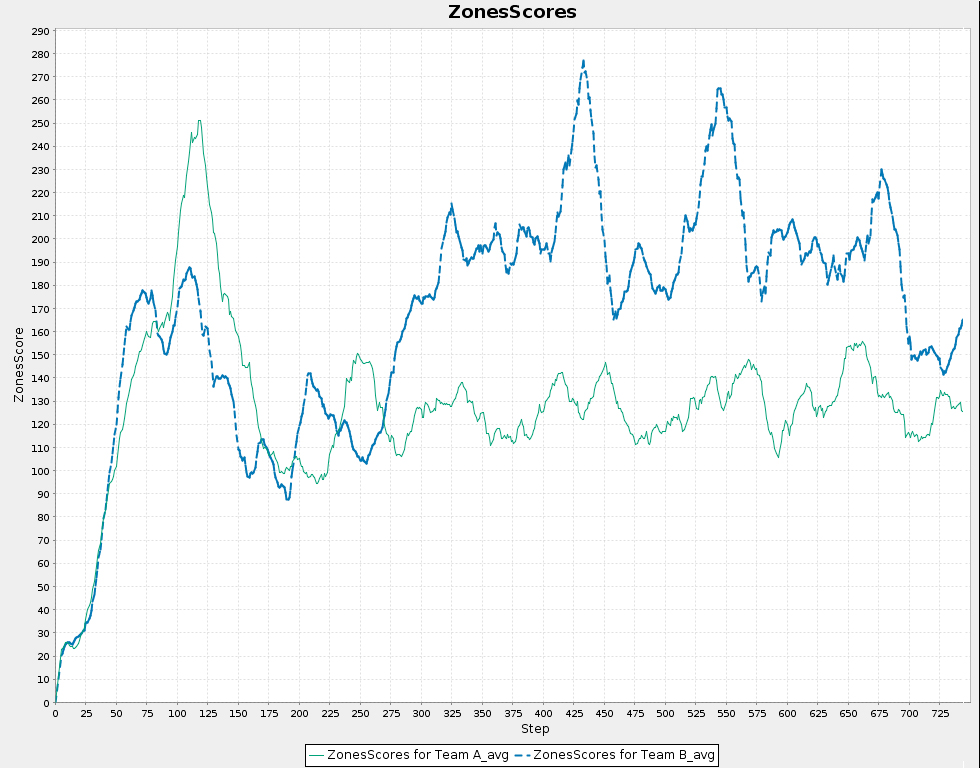
\includegraphics[width=0.48\linewidth]{./zones1.jpg}\label{zones1}}
	\hspace{0cm} % este comando é para deixar uma distância de 1 cm entre as figuras
	\subfloat[]{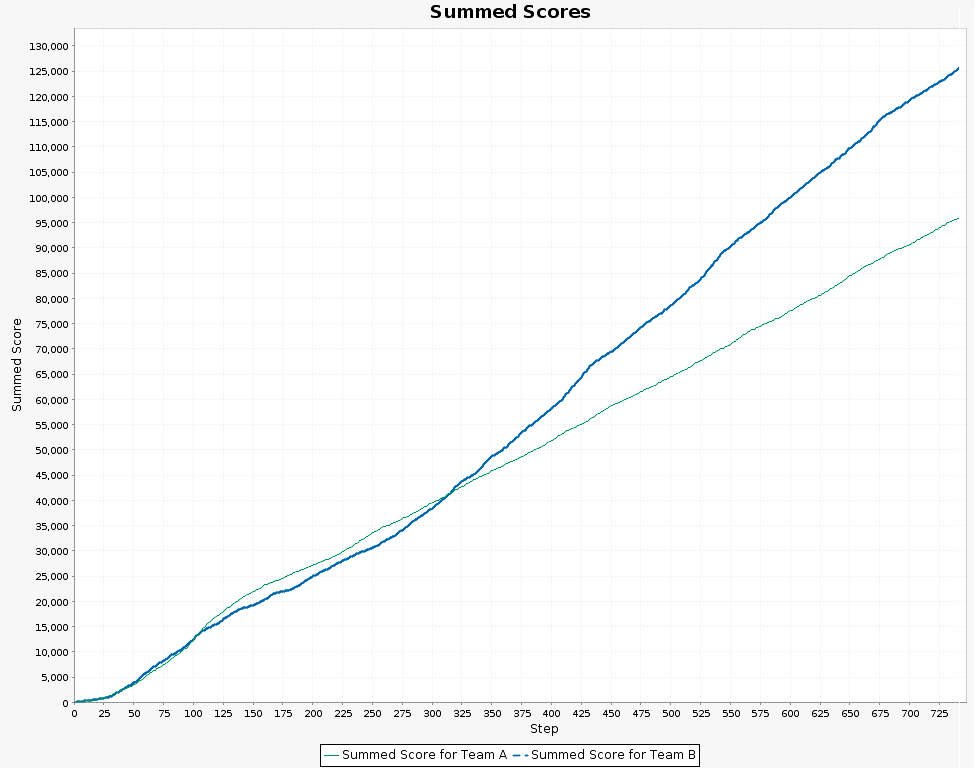
\includegraphics[width=0.48\linewidth]{./zones2.jpg}\label{zones2}}
	\caption{The green system tries to conquer one single zone and the blue system looks for two zones. The blue system finishes the match with a highest score because it keeps scoring in a zone without disputing it with opponents.}
	\label{fig:1x2morrinho}
\end{figure} 

% talvez incluir numa nova versao:
% - problema de processar percepcao
% - tempos de processamento, desempenho do time
% - gargalos
% - profilling, e avaliacoes nossoas
% - colocar umas telas do cenario que sejam significativas

